%\documentclass[12pt]{beamer}
\documentclass[12pt,envcountsect, leqno,xcolor=dvipsnames]{beamer}
\mode<presentation>
\setbeameroption{hide notes}
%\usepackage[utf8]{inputenc}
\usepackage{hyperref}
\usepackage{amssymb}
\usepackage{amsmath}
%\usepackage{mathpazo}
%\usepackage{multimedia}
\usepackage{amsfonts}
\usepackage{graphicx}
\usepackage{natbib}
\usepackage{setspace}
%\usepackage{multirow}
\usepackage{color}
\usepackage{array}
%\usepackage{booktabs}
\usepackage{colortbl,xcolor}
\usepackage{tikz}
 \usepackage{booktabs}
 \usepackage{longtable}
 \usepackage{multirow}
\usepackage{caption}
\usepackage{subcaption}

 \usetikzlibrary{decorations.markings}

\tikzset{->-/.style={decoration={
  markings,
  mark=at position .5 with {\arrow{>}}},postaction={decorate}}}

  \tikzset{-<-/.style={decoration={
  markings,
  mark=at position .5 with {\arrow{<}}},postaction={decorate}}}

%\usepackage{xfrac}
%\newcolumntype{L}[1]{>{\raggedright\let\newline\\\arraybackslash\hspace{0pt}}m{#1}}
%\newcolumntype{C}[1]{>{\centering\let\newline\\\arraybackslash\hspace{0pt}}m{#1}}
%\newcolumntype{R}[1]{>{\raggedleft\let\newline\\\arraybackslash\hspace{0pt}}m{#1}}

\frenchspacing
%\usepackage[thicklines,makeroom]{cancel}


\newtheorem{proposition}{Proposition}
\usetheme{Boadilla}

\newcommand{\bi}{\begin{itemize}}
\newcommand{\ei}{\end{itemize}}
\newcommand{\bn}{\begin{enumerate}}
\newcommand{\en}{\end{enumerate}}
\newcommand{\tcm}{\textcolor{magenta}}


\setbeamertemplate{enumerate items}[default]
\setbeamertemplate{navigation symbols}{} %remove navigation symbols

\title[]{}

\author[]{
\\
{\footnotesize Federal Reserve Bank of New York}
}
\date{March 2018}

\makeatother
\title[Empirical Network Contagion]{Empirical Network Contagion for U.S. Financial Institutions}
\author[Duarte and Jones]{Fernando Duarte and Collin Jones} 
\institute[NY Fed]{Federal Reserve Bank of New York and Federal Reserve Bank of New York}
\date{March 2018}
\renewcommand{\baselinestretch}{1.2}
\AtBeginSection[]
{
  \begin{frame}<beamer>
    \frametitle{Outline}
    \tableofcontents[currentsection]
  \end{frame}
}
%\titlegraphic{\includegraphics[width=\textwidth,height=\textheight]{XXX.pdf}}
\definecolor{Highlight}{HTML}{C71585}


\begin{document}


\begin{frame}[plain]

\titlepage


\begin{scriptsize} \begin{center}
The views expressed in this presentation are those of the authors and are
not necessarily reflective of views at the Federal Reserve Bank of
New York or the Federal Reserve System.
\end{center} \end{scriptsize}

\end{frame}

\setcounter{framenumber}{0}
   \setbeamertemplate{footline}{%
       \raisebox{5pt}{\makebox[\paperwidth]{\hfill\makebox[10pt]{\scriptsize\insertframenumber}}}}



\begin{frame}{Motivation} \setstretch{1.2}

\bi
\item Explosion of research on financial networks since crisis
\item Problem: lack of data
	\bi
	\item Literature predominantly theory
	\item Empirics limited to subsector or single asset class
	\item Simulations to fill in for missing data
	\item Or top-down using non-network data (CoVaR, srisk, etc.)
	\ei 
\item Network contagion: direct or indirect connections?
	\bi
	\item Fire sales: indirect connection through overlap in assets
	\item Default spillovers: direct counter-party risk
	\item Other?
	\ei
\ei

\end{frame}

\begin{frame}{This paper: Empirical Default Spillovers} \setstretch{1.2}
\bi
\item  Empirically  estimate  a  measure  of  expected network default spillovers for entire US financial system 2002-2016
\item Network model of Eisenberg and Noe (2001)
	\bn
	\item Nodes are financial institutions; hold in- and out-of-network assets and liabilities
	\item Shocks to outside assets can cause a node to default
	\item Default of a node can trigger default of counter-parties
	\en 
\item Estimating default spillovers requires all bilateral contracts
\ei
\end{frame}

\begin{frame}{This paper: Empirical Default Spillovers} \setstretch{1.2}
\bi
\item Glasserman and Young (2015): an \textbf{upper bound} on spillovers only requires \textbf{node-specific} data
	\bi
	\item Outside assets, ratio of inside liabilities to total liabilities, probability of default
	\ei
\item Check tightness of upper bound by creating worst network given empirical node-dependent data
\ei
\end{frame}

\begin{frame}{Main Result: Network Spillovers Can Be Large}
\begin{center}
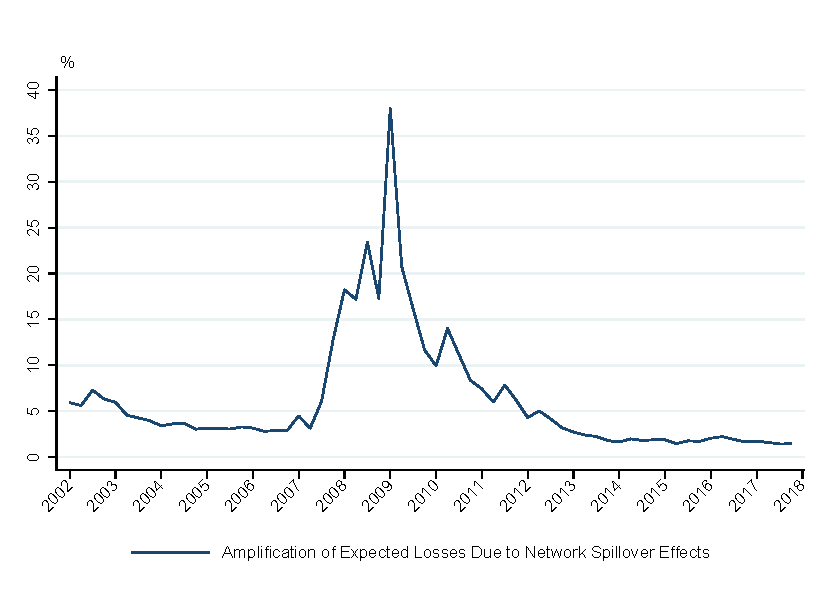
\includegraphics[width=\linewidth, height=0.8\textheight,keepaspectratio]{../output/NVI_benchmark.pdf}
\end{center}

\end{frame}

\begin{frame}{Outline of This Talk} \setstretch{1.5}
\bn
\item Network model and upper bound on spillovers
\item Data and estimate of upper bound
\item Decompositions, robustness
\item Worst and best networks given empirical data
\en
\end{frame}

\begin{frame}

{\Large Network model and upper bound on spillovers}

\end{frame}


\begin{frame}{A Simple Example} \setstretch{1.2}

\begin{center}
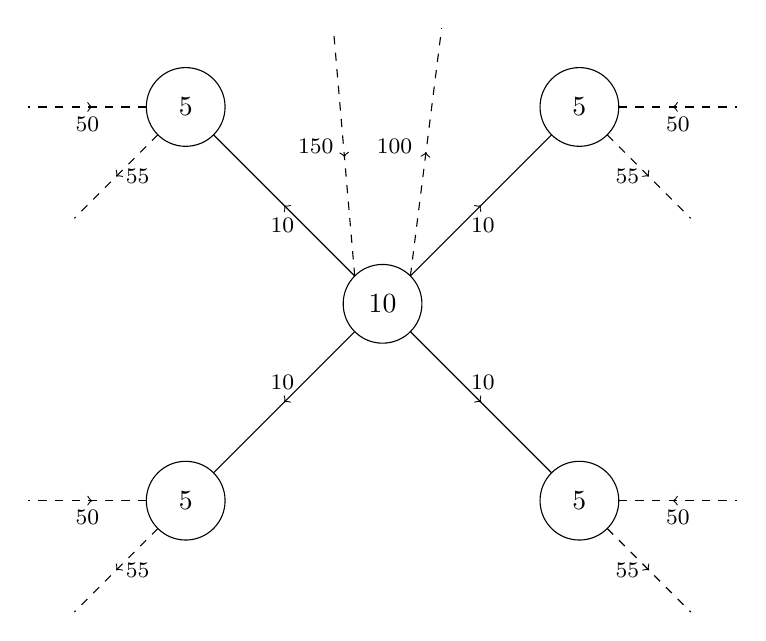
\begin{tikzpicture}[xscale=.5, yscale=.5]

\draw (5, 5) circle [radius=1];
\node at (5,5) {$10$};
\draw (10, 10) circle [radius=1];
\node at (10,10) {$5$};
\draw (10, 0) circle [radius=1];
\node at (10,0) {$5$};
\draw (0, 10) circle [radius=1];
\node at (0,10) {$5$};
\draw (0, 0) circle [radius=1];
\node at (0,0) {$5$};

\draw[dashed, -<-] (-1, 10) -- (-4, 10);
\draw[dashed, ->-] (-.7071, 9.2929) -- (-2.82843, 7.171573);
\node [below] at (-2.5, 10) {\footnotesize $50$};
\node [right] at (-1.76777, 8.232233) {\footnotesize $55$};

\draw[dashed, -<-] (-1, 0) -- (-4, 0);
\draw[dashed, ->-] (-.7071, -.7071) -- (-2.82843, -2.82843);
\node [below] at (-2.5, 0) {\footnotesize $50$};
\node [right] at (-1.76777, -1.76777) {\footnotesize $55$};

\draw[dashed, -<-] (11, 10) -- (14, 10);
\draw[dashed, ->-] (10.7071, 9.2929) -- (12.82843, 7.171573);
\node [below] at (12.5, 10) {\footnotesize $50$};
\node [left] at (11.76777, 8.232233) {\footnotesize $55$};

\draw[dashed, -<-] (11, 0) -- (14, 0);
\draw[dashed, ->-] (10.7071, -.7071) -- (12.82843, -2.82843);
\node [below] at (12.5, 0) {\footnotesize $50$};
\node [left] at (11.76777, -1.76777) {\footnotesize $55$};

\draw[dashed, -<-] (4.2929, 5.7071) -- (3.75, 12);
\draw[->-] (4.2929, 5.7071) -- (.7071, 9.2929);
\draw[dashed,  ->-] (5.7071, 5.7071) -- (6.5, 12);
\draw[->-] (5.7071, 5.7071) -- (9.2929, 9.2929);
\draw[->-] (4.2929, 4.2929) -- (.7071, .7071);
\draw[->-] (5.7071, 4.2929) -- (9.2929, .7071);
\node [left] at (4, 9) {\footnotesize $150$};
\node [left] at (6, 9) {\footnotesize $100$};
\node [left] at (3, 7) {\footnotesize $10$};
\node [right] at (7, 7) {\footnotesize $10$};
\node [left] at (3, 3) {\footnotesize $10$};
\node [right] at (7, 3) {\footnotesize $10$};
\end{tikzpicture}

\end{center}

\end{frame}

%1
\begin{frame}{A Simple Example: Losses} \setstretch{1.2}
\begin{center}
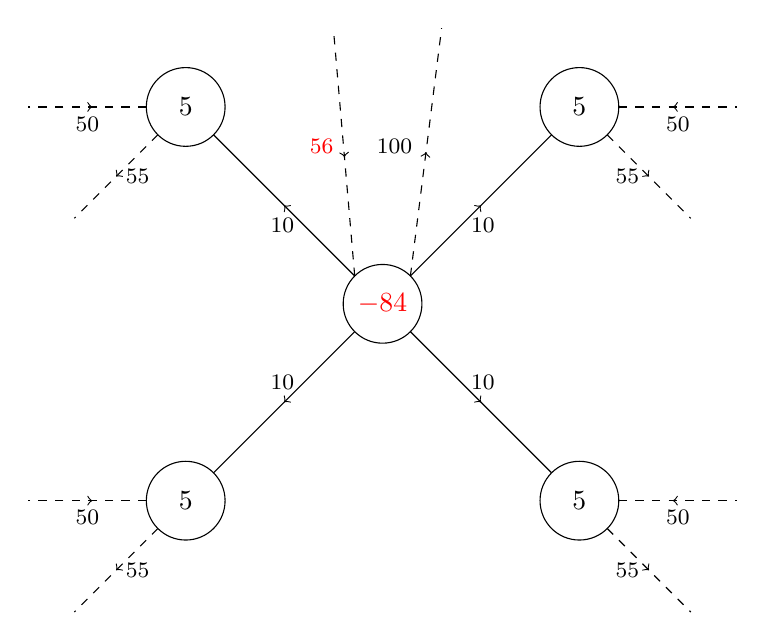
\begin{tikzpicture}[xscale=.5, yscale=.5]

\draw (5, 5) circle [radius=1];
\node at (5,5) {\textcolor{red}{$-84$}};
\draw (10, 10) circle [radius=1];
\node at (10,10) {$5$};
\draw (10, 0) circle [radius=1];
\node at (10,0) {$5$};
\draw (0, 10) circle [radius=1];
\node at (0,10) {$5$};
\draw (0, 0) circle [radius=1];
\node at (0,0) {$5$};

\draw[dashed, -<-] (-1, 10) -- (-4, 10);
\draw[dashed, ->-] (-.7071, 9.2929) -- (-2.82843, 7.171573);
\node [below] at (-2.5, 10) {\footnotesize $50$};
\node [right] at (-1.76777, 8.232233) {\footnotesize $55$};

\draw[dashed, -<-] (-1, 0) -- (-4, 0);
\draw[dashed, ->-] (-.7071, -.7071) -- (-2.82843, -2.82843);
\node [below] at (-2.5, 0) {\footnotesize $50$};
\node [right] at (-1.76777, -1.76777) {\footnotesize $55$};

\draw[dashed, -<-] (11, 10) -- (14, 10);
\draw[dashed, ->-] (10.7071, 9.2929) -- (12.82843, 7.171573);
\node [below] at (12.5, 10) {\footnotesize $50$};
\node [left] at (11.76777, 8.232233) {\footnotesize $55$};

\draw[dashed, -<-] (11, 0) -- (14, 0);
\draw[dashed, ->-] (10.7071, -.7071) -- (12.82843, -2.82843);
\node [below] at (12.5, 0) {\footnotesize $50$};
\node [left] at (11.76777, -1.76777) {\footnotesize $55$};

\draw[dashed, -<-] (4.2929, 5.7071) -- (3.75, 12);
\draw[->-] (4.2929, 5.7071) -- (.7071, 9.2929);
\draw[dashed,  ->-] (5.7071, 5.7071) -- (6.5, 12);
\draw[->-] (5.7071, 5.7071) -- (9.2929, 9.2929);
\draw[->-] (4.2929, 4.2929) -- (.7071, .7071);
\draw[->-] (5.7071, 4.2929) -- (9.2929, .7071);
\node [left] at (4, 9) {\textcolor{red}{\footnotesize $56$}};
\node [left] at (6, 9) {\footnotesize $100$};
\node [left] at (3, 7) {\footnotesize $10$};
\node [right] at (7, 7) {\footnotesize $10$};
\node [left] at (3, 3) {\footnotesize $10$};
\node [right] at (7, 3) {\footnotesize $10$};
\end{tikzpicture}
\end{center}

\end{frame}
%2
\begin{frame}{A Simple Example: Losses After Shock} \setstretch{1.2}
\begin{center}
\begin{tikzpicture}[xscale=.5, yscale=.5]

\draw (5, 5) circle [radius=1];
\node at (5,5) {$0$};
\draw (10, 10) circle [radius=1];
\node at (10,10) {\textcolor{red}{$-1$}};
\draw (10, 0) circle [radius=1];
\node at (10,0) {\textcolor{red}{$-1$}};
\draw (0, 10) circle [radius=1];
\node at (0,10) {\textcolor{red}{$-1$}};
\draw (0, 0) circle [radius=1];
\node at (0,0) {\textcolor{red}{$-1$}};

\draw[dashed, -<-] (-1, 10) -- (-4, 10);
\draw[dashed, ->-] (-.7071, 9.2929) -- (-2.82843, 7.171573);
\node [below] at (-2.5, 10) {\footnotesize $50$};
\node [right] at (-1.76777, 8.232233) {\footnotesize $55$};

\draw[dashed, -<-] (-1, 0) -- (-4, 0);
\draw[dashed, ->-] (-.7071, -.7071) -- (-2.82843, -2.82843);
\node [below] at (-2.5, 0) {\footnotesize $50$};
\node [right] at (-1.76777, -1.76777) {\footnotesize $55$};

\draw[dashed, -<-] (11, 10) -- (14, 10);
\draw[dashed, ->-] (10.7071, 9.2929) -- (12.82843, 7.171573);
\node [below] at (12.5, 10) {\footnotesize $50$};
\node [left] at (11.76777, 8.232233) {\footnotesize $55$};

\draw[dashed, -<-] (11, 0) -- (14, 0);
\draw[dashed, ->-] (10.7071, -.7071) -- (12.82843, -2.82843);
\node [below] at (12.5, 0) {\footnotesize $50$};
\node [left] at (11.76777, -1.76777) {\footnotesize $55$};

\draw[dashed, -<-] (4.2929, 5.7071) -- (3.75, 12);
\draw[->-] (4.2929, 5.7071) -- (.7071, 9.2929);
\draw[dashed,  ->-] (5.7071, 5.7071) -- (6.5, 12);
\draw[->-] (5.7071, 5.7071) -- (9.2929, 9.2929);
\draw[->-] (4.2929, 4.2929) -- (.7071, .7071);
\draw[->-] (5.7071, 4.2929) -- (9.2929, .7071);
\node [left] at (4, 9) {\footnotesize $56$};
\node [left] at (6, 9) {\textcolor{red}{\footnotesize $40$}};
\node [left] at (3, 7) {\textcolor{red}{\footnotesize $4$}};
\node [right] at (7, 7) {\textcolor{red}{\footnotesize $4$}};
\node [left] at (3, 3) {\textcolor{red}{\footnotesize $4$}};
\node [right] at (7, 3) {\textcolor{red}{\footnotesize $4$}};
\end{tikzpicture}
\end{center}

\end{frame}

%3
\begin{frame}{A Simple Example: Default Contagion} \setstretch{1.2}
\begin{center}
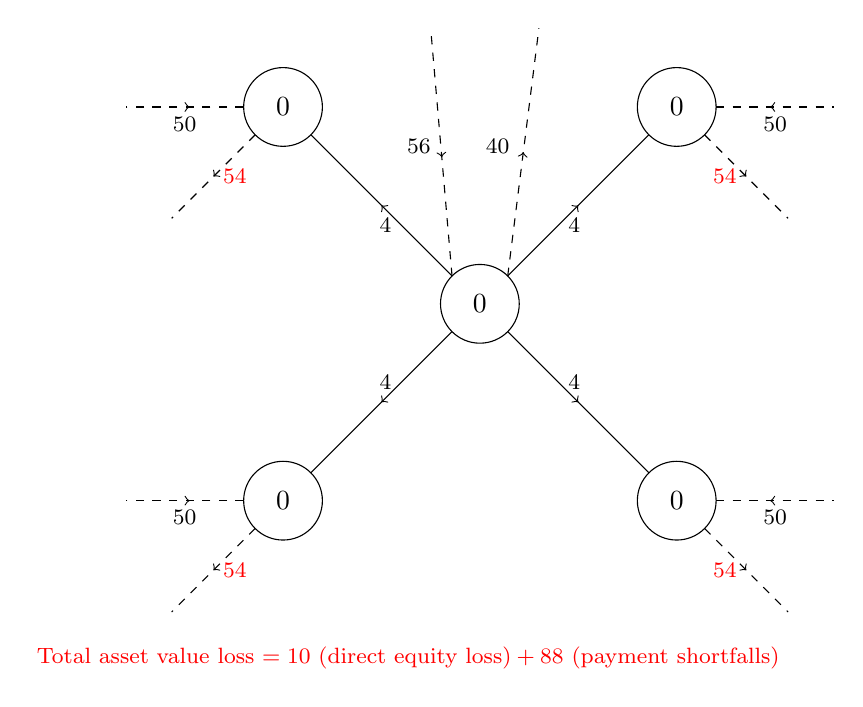
\begin{tikzpicture}[xscale=.5, yscale=.5]

\draw (5, 5) circle [radius=1];
\node at (5,5) {$0$};
\draw (10, 10) circle [radius=1];
\node at (10,10) {$0$};
\draw (10, 0) circle [radius=1];
\node at (10,0) {$0$};
\draw (0, 10) circle [radius=1];
\node at (0,10) {$0$};
\draw (0, 0) circle [radius=1];
\node at (0,0) {$0$};

\draw[dashed, -<-] (-1, 10) -- (-4, 10);
\draw[dashed, ->-] (-.7071, 9.2929) -- (-2.82843, 7.171573);
\node [below] at (-2.5, 10) {\footnotesize $50$};
\node [right] at (-1.76777, 8.232233) {\textcolor{red}{\footnotesize $54$}};

\draw[dashed, -<-] (-1, 0) -- (-4, 0);
\draw[dashed, ->-] (-.7071, -.7071) -- (-2.82843, -2.82843);
\node [below] at (-2.5, 0) {\footnotesize $50$};
\node [right] at (-1.76777, -1.76777) {\textcolor{red}{\footnotesize $54$}};

\draw[dashed, -<-] (11, 10) -- (14, 10);
\draw[dashed, ->-] (10.7071, 9.2929) -- (12.82843, 7.171573);
\node [below] at (12.5, 10) {\footnotesize $50$};
\node [left] at (11.76777, 8.232233) {\textcolor{red}{\footnotesize $54$}};

\draw[dashed, -<-] (11, 0) -- (14, 0);
\draw[dashed, ->-] (10.7071, -.7071) -- (12.82843, -2.82843);
\node [below] at (12.5, 0) {\footnotesize $50$};
\node [left] at (11.76777, -1.76777) {\textcolor{red}{\footnotesize $54$}};

\draw[dashed, -<-] (4.2929, 5.7071) -- (3.75, 12);
\draw[->-] (4.2929, 5.7071) -- (.7071, 9.2929);
\draw[dashed,  ->-] (5.7071, 5.7071) -- (6.5, 12);
\draw[->-] (5.7071, 5.7071) -- (9.2929, 9.2929);
\draw[->-] (4.2929, 4.2929) -- (.7071, .7071);
\draw[->-] (5.7071, 4.2929) -- (9.2929, .7071);
\node [left] at (4, 9) {\footnotesize $56$};
\node [left] at (6, 9) {\footnotesize $40$};
\node [left] at (3, 7) {\footnotesize $4$};
\node [right] at (7, 7) {\footnotesize $4$};
\node [left] at (3, 3) {\footnotesize $4$};
\node [right] at (7, 3) {\footnotesize $4$};

\node [right] at (-6.5, -4) {\textcolor{red}{\footnotesize Total asset value loss $= 10 \text{ (direct equity loss)} + 88 \text{ (payment shortfalls)}$}};

\end{tikzpicture}
\end{center}

\end{frame}

\begin{frame}{The Disconnected Network: Losses} \setstretch{1.2}

\begin{center}
\begin{tikzpicture}[xscale=.5, yscale=.5]

\draw (5, 5) circle [radius=1];
\node at (5,5) {$10$};
\draw (10, 10) circle [radius=1];
\node at (10,10) {$5$};
\draw (10, 0) circle [radius=1];
\node at (10,0) {$5$};
\draw (0, 10) circle [radius=1];
\node at (0,10) {$5$};
\draw (0, 0) circle [radius=1];
\node at (0,0) {$5$};

\draw[dashed, -<-] (-1, 10) -- (-4, 10);
\draw[dotted, -<-] (-1, 10) -- (-4, 11.5);
\draw[dashed, ->-] (-.7071, 9.2929) -- (-2.82843, 7.171573);
\node [below] at (-2.5, 10) {\footnotesize $50$};
\node [right] at (-1.76777, 8.232233) {\footnotesize $55$};
\node [above] at (-2.5, 11) {\footnotesize $10$};

\draw[dashed, -<-] (-1, 0) -- (-4, 0);
\draw[dotted, -<-] (-1, 0) -- (-4, 1.5);
\draw[dashed, ->-] (-.7071, -.7071) -- (-2.82843, -2.82843);
\node [below] at (-2.5, 0) {\footnotesize $50$};
\node [right] at (-1.76777, -1.76777) {\footnotesize $55$};
\node [above] at (-2.5, 1) {\footnotesize $10$};

\draw[dashed, -<-] (11, 10) -- (14, 10);
\draw[dotted, -<-] (11, 10) -- (14, 11.5);
\draw[dashed, ->-] (10.7071, 9.2929) -- (12.82843, 7.171573);
\node [below] at (12.5, 10) {\footnotesize $50$};
\node [above] at (12.5, 11) {\footnotesize $10$};
\node [left] at (11.76777, 8.232233) {\footnotesize $55$};

\draw[dashed, -<-] (11, 0) -- (14, 0);
\draw[dotted, -<-] (11, 0) -- (14, 1.5);
\draw[dashed, ->-] (10.7071, -.7071) -- (12.82843, -2.82843);AH
\node [below] at (12.5, 0) {\footnotesize $50$};
\node [above] at (12.5, 1) {\footnotesize $10$};
\node [left] at (11.76777, -1.76777) {\footnotesize $55$};

\draw[dashed, -<-] (4.2929, 5.7071) -- (4, 12);
\draw[dashed, ->-] (5.7071, 5.7071) -- (6, 12);
\draw[dotted, ->-] (5.7071, 5.7071) -- (8, 12);
\node [left] at (4.25, 9) {\footnotesize $150$};
\node [left] at (6, 9) {\footnotesize $100$};
\node [right] at (6.5, 8) {\footnotesize $40$};

\end{tikzpicture}

\end{center}

\end{frame}

%1
\begin{frame}{The Disconnected Network} \setstretch{1.2}

\begin{center}
\begin{tikzpicture}[xscale=.5, yscale=.5]

\draw (5, 5) circle [radius=1];
\node at (5,5) {\textcolor{red}{$-84$}};
\draw (10, 10) circle [radius=1];
\node at (10,10) {$5$};
\draw (10, 0) circle [radius=1];
\node at (10,0) {$5$};
\draw (0, 10) circle [radius=1];
\node at (0,10) {$5$};
\draw (0, 0) circle [radius=1];
\node at (0,0) {$5$};

\draw[dashed, -<-] (-1, 10) -- (-4, 10);
\draw[dotted, -<-] (-1, 10) -- (-4, 11.5);
\draw[dashed, ->-] (-.7071, 9.2929) -- (-2.82843, 7.171573);
\node [below] at (-2.5, 10) {\footnotesize $50$};
\node [right] at (-1.76777, 8.232233) {\footnotesize $55$};
\node [above] at (-2.5, 11) {\footnotesize $10$};

\draw[dashed, -<-] (-1, 0) -- (-4, 0);
\draw[dotted, -<-] (-1, 0) -- (-4, 1.5);
\draw[dashed, ->-] (-.7071, -.7071) -- (-2.82843, -2.82843);
\node [below] at (-2.5, 0) {\footnotesize $50$};
\node [right] at (-1.76777, -1.76777) {\footnotesize $55$};
\node [above] at (-2.5, 1) {\footnotesize $10$};

\draw[dashed, -<-] (11, 10) -- (14, 10);
\draw[dotted, -<-] (11, 10) -- (14, 11.5);
\draw[dashed, ->-] (10.7071, 9.2929) -- (12.82843, 7.171573);
\node [below] at (12.5, 10) {\footnotesize $50$};
\node [above] at (12.5, 11) {\footnotesize $10$};
\node [left] at (11.76777, 8.232233) {\footnotesize $55$};

\draw[dashed, -<-] (11, 0) -- (14, 0);
\draw[dotted, -<-] (11, 0) -- (14, 1.5);
\draw[dashed, ->-] (10.7071, -.7071) -- (12.82843, -2.82843);
\node [below] at (12.5, 0) {\footnotesize $50$};
\node [above] at (12.5, 1) {\footnotesize $10$};
\node [left] at (11.76777, -1.76777) {\footnotesize $55$};

\draw[dashed, -<-] (4.2929, 5.7071) -- (4, 12);
\draw[dashed, ->-] (5.7071, 5.7071) -- (6, 12);
\draw[dotted, ->-] (5.7071, 5.7071) -- (8, 12);
\node [left] at (4.25, 9) {\textcolor{red}{\footnotesize $56$}};
\node [left] at (6, 9) {\footnotesize $100$};
\node [right] at (6.5, 8) {\footnotesize $40$};

\end{tikzpicture}


\end{center}
\end{frame}
%2
\begin{frame}{The Disconnected Network: No Contagion} \setstretch{1.2}

\begin{center}
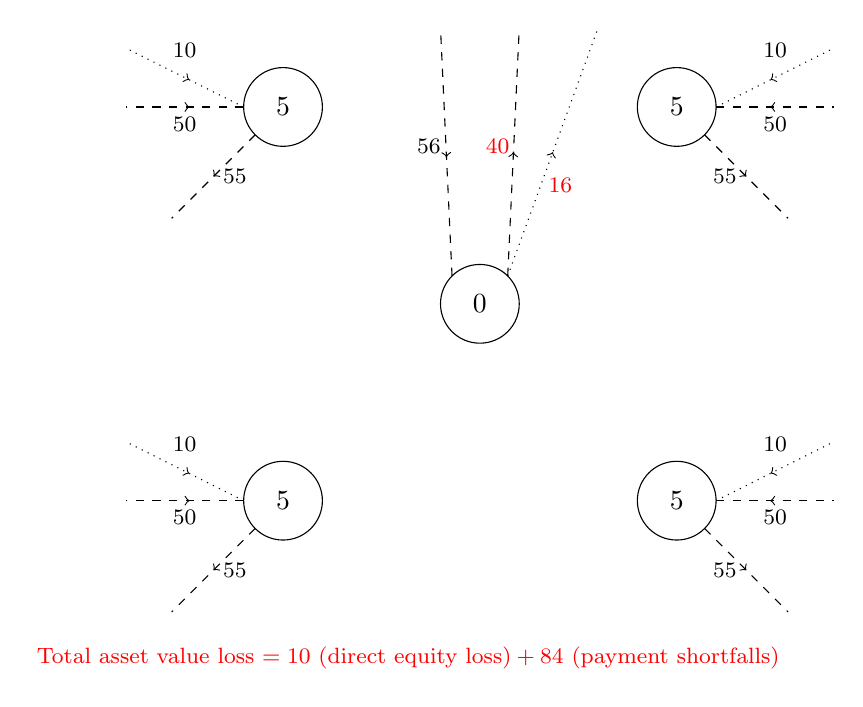
\begin{tikzpicture}[xscale=.5, yscale=.5]

\draw (5, 5) circle [radius=1];
\node at (5,5) {$0$};
\draw (10, 10) circle [radius=1];
\node at (10,10) {$5$};
\draw (10, 0) circle [radius=1];
\node at (10,0) {$5$};
\draw (0, 10) circle [radius=1];
\node at (0,10) {$5$};
\draw (0, 0) circle [radius=1];
\node at (0,0) {$5$};

\draw[dashed, -<-] (-1, 10) -- (-4, 10);
\draw[dotted, -<-] (-1, 10) -- (-4, 11.5);
\draw[dashed, ->-] (-.7071, 9.2929) -- (-2.82843, 7.171573);
\node [below] at (-2.5, 10) {\footnotesize $50$};
\node [right] at (-1.76777, 8.232233) {\footnotesize $55$};
\node [above] at (-2.5, 11) {\footnotesize $10$};

\draw[dashed, -<-] (-1, 0) -- (-4, 0);
\draw[dotted, -<-] (-1, 0) -- (-4, 1.5);
\draw[dashed, ->-] (-.7071, -.7071) -- (-2.82843, -2.82843);
\node [below] at (-2.5, 0) {\footnotesize $50$};
\node [right] at (-1.76777, -1.76777) {\footnotesize $55$};
\node [above] at (-2.5, 1) {\footnotesize $10$};

\draw[dashed, -<-] (11, 10) -- (14, 10);
\draw[dotted, -<-] (11, 10) -- (14, 11.5);
\draw[dashed, ->-] (10.7071, 9.2929) -- (12.82843, 7.171573);
\node [below] at (12.5, 10) {\footnotesize $50$};
\node [above] at (12.5, 11) {\footnotesize $10$};
\node [left] at (11.76777, 8.232233) {\footnotesize $55$};

\draw[dashed, -<-] (11, 0) -- (14, 0);
\draw[dotted, -<-] (11, 0) -- (14, 1.5);
\draw[dashed, ->-] (10.7071, -.7071) -- (12.82843, -2.82843);
\node [below] at (12.5, 0) {\footnotesize $50$};
\node [above] at (12.5, 1) {\footnotesize $10$};
\node [left] at (11.76777, -1.76777) {\footnotesize $55$};

\draw[dashed, -<-] (4.2929, 5.7071) -- (4, 12);
\draw[dashed, ->-] (5.7071, 5.7071) -- (6, 12);
\draw[dotted, ->-] (5.7071, 5.7071) -- (8, 12);
\node [left] at (4.25, 9) {\footnotesize $56$};
\node [left] at (6, 9) {\textcolor{red}{\footnotesize $40$}};
\node [right] at (6.5, 8) {\textcolor{red}{\footnotesize $16$}};

\node [right] at (-6.5, -4) {\textcolor{red}{\footnotesize Total asset value loss $= 10 \text{ (direct equity loss)} + 84 \text{ (payment shortfalls)}$}};

\end{tikzpicture}


\end{center}

\end{frame}

\begin{frame}{A Fixed Point Example} \setstretch{1.2}

\begin{center}
\begin{center}
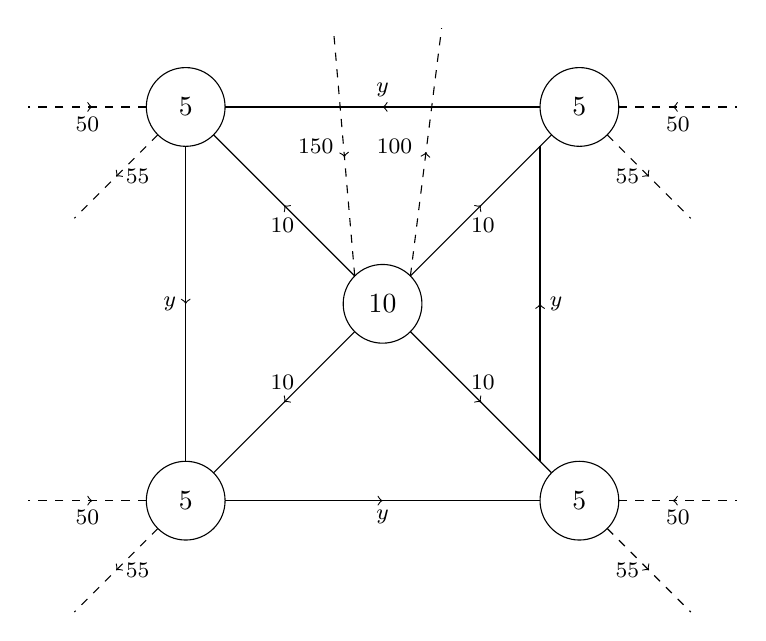
\begin{tikzpicture}[xscale=.5, yscale=.5]

\draw (5, 5) circle [radius=1];
\node at (5,5) {$10$};
\draw (10, 10) circle [radius=1];
\node at (10,10) {$5$};
\draw (10, 0) circle [radius=1];
\node at (10,0) {$5$};
\draw (0, 10) circle [radius=1];
\node at (0,10) {$5$};
\draw (0, 0) circle [radius=1];
\node at (0,0) {$5$};

\draw[dashed, -<-] (-1, 10) -- (-4, 10);
\draw[dashed, ->-] (-.7071, 9.2929) -- (-2.82843, 7.171573);
\node [below] at (-2.5, 10) {\footnotesize $50$};
\node [right] at (-1.76777, 8.232233) {\footnotesize $55$};

\draw[dashed, -<-] (-1, 0) -- (-4, 0);
\draw[dashed, ->-] (-.7071, -.7071) -- (-2.82843, -2.82843);
\node [below] at (-2.5, 0) {\footnotesize $50$};
\node [right] at (-1.76777, -1.76777) {\footnotesize $55$};

\draw[dashed, -<-] (11, 10) -- (14, 10);
\draw[dashed, ->-] (10.7071, 9.2929) -- (12.82843, 7.171573);
\node [below] at (12.5, 10) {\footnotesize $50$};
\node [left] at (11.76777, 8.232233) {\footnotesize $55$};

\draw[dashed, -<-] (11, 0) -- (14, 0);
\draw[dashed, ->-] (10.7071, -.7071) -- (12.82843, -2.82843);
\node [below] at (12.5, 0) {\footnotesize $50$};
\node [left] at (11.76777, -1.76777) {\footnotesize $55$};

\draw[dashed, -<-] (4.2929, 5.7071) -- (3.75, 12);
\draw[->-] (4.2929, 5.7071) -- (.7071, 9.2929);
\draw[dashed,  ->-] (5.7071, 5.7071) -- (6.5, 12);
\draw[->-] (5.7071, 5.7071) -- (9.2929, 9.2929);
\draw[->-] (4.2929, 4.2929) -- (.7071, .7071);
\draw[->-] (5.7071, 4.2929) -- (9.2929, .7071);
\node [left] at (4, 9) {\footnotesize $150$};
\node [left] at (6, 9) {\footnotesize $100$};
\node [left] at (3, 7) {\footnotesize $10$};
\node [right] at (7, 7) {\footnotesize $10$};
\node [left] at (3, 3) {\footnotesize $10$};
\node [right] at (7, 3) {\footnotesize $10$};

\draw[->-] (0, 9) -- (0, 1);
\node [left] at (0, 5) {\footnotesize $y$};
\draw[->-] (1, 0) -- (9, 0);
\node [below] at (5, 0) {\footnotesize $y$};
\draw[->-] (9, 1) -- (9, 9);
\node [right] at (9, 5) {\footnotesize $y$};
\draw[->-] (9, 10) -- (1, 10);
\node [above] at (5, 10) {\footnotesize $y$};

\end{tikzpicture}
\end{center}
\end{center}

\end{frame}

\begin{frame}{Default Spillovers and an Upper Bound} \setstretch{1.2}

\bi
\item Want to measure $R=\mathbb{E}[Loss_{\text{actual}}] / \mathbb{E}[Loss_\text{disconnected}]$
\item Instead, find bound B
	\[
	R \leq B=1+\frac{1}{(1-\beta ^{+})} \frac{\sum_{i \in S} {\delta _{i}c_{i}}}{\sum_{i \in S}{c_{i}}}\vspace{-0.1in}
	\]
where\vspace{-0.1in}
\begin{eqnarray*}
\delta _{i} &:&\text{probability of default for }i\\
c_{i} &:&\text{dollar value of outside assets for }i\\
\beta ^{+} &:& \beta^{+}=\max_{i \in S}\beta _{i} \\
\beta_i &:&i\text{'s in-network liabilities relative to total liabilities}\\
S &:&\text{Set of nodes in network}
\end{eqnarray*}%

\ei

\end{frame}


\begin{frame}{Default Spillovers and an Upper Bound} \setstretch{1.2}

\bi
\item Define the \textit{Network Vulnerability Index} NVI$= B-1$
\item Decomposition of NVI
	\[
	\text{NVI} = \underbrace{\frac{1}{1-\beta ^{+}}}_{\substack{\text{Connectivity}  \\ \text{multiplier}}} \times \underbrace{\frac{\sum_{i \in S} {\delta _{i}c_{i}}}{\sum_{i \in S}{c_{i}}}}_{\substack{\text{Avg default} \\ \text{prob}}}
	\]
\item Node \textit{contagion index}: maximum shortfall that a node can pass on to network
	\[
	\text{contagion index} = w_i \beta_i \lambda_i
	\]
\ei
\hspace{0.35in}where $\lambda_i=\frac{c_i}{w_i}$ is the leverage of $i$'s outside assets. 
\end{frame}

\begin{frame}

{\Large Data and estimate of upper bound}

\end{frame}



\begin{frame}{Data Sources} \setstretch{1.2}

\bi
\item Bank holding companies: Y-9C 
\item Insured Deposits: Call Report
\item Broker-dealers: Focus Report (aggregated by tier 1-10, etc)
\item Hedge Funds: HFR (not yet done, sub-universe)
\item Other traded firms: Moody's Analytics
\item Other firms and aggregates: Financial Accounts of U.S. (FOF)
\item Probabilities of default: Moody's Analytics (KMV)
\item Time of bankruptcy: Moody's Default and Recovery Database
\ei
\end{frame}

\begin{frame}{Coverage is Large}

\begin{center}
\includegraphics[width = \textwidth, height=0.9\textheight,keepaspectratio]{../output/coverage_broad.pdf}
\end{center}

\end{frame}


\begin{frame}{Distribution of Assets: BHC dominate} \setstretch{1.2}
\begin{center}
\includegraphics[width = \textwidth, height=0.9\textheight,keepaspectratio]{../output/ffunds_assets_area}
\end{center}

\end{frame}

\begin{frame}{Classification of BHC Assets}

\begin{table} [H]\centering \scriptsize
%\def\sym#1{\ifmmode^{#1}\else\(^{#1}\)\fi}
\begin{minipage}{.48\textwidth}
\setlength{\tabcolsep}{12pt}
\input{../output/asset_in_formatted}
\end{minipage}%
\begin{minipage}{.48\textwidth}
\input{../output/asset_out_formatted}
\end{minipage}
\centering
\end{table}

\end{frame}

\begin{frame}{Classification of BHC Liabilities} \setstretch{1.2}

\begin{table} [H]\centering \scriptsize
%\def\sym#1{\ifmmode^{#1}\else\(^{#1}\)\fi}
\begin{minipage}{.48\textwidth}
\setlength{\tabcolsep}{10pt}
\input{../output/liab_in_formatted}
\end{minipage}
\begin{minipage}{.48\textwidth}
\setlength{\tabcolsep}{12pt}
\input{../output/liab_out_formatted}
\end{minipage}
\end{table}

\end{frame}


%\begin{frame}{Classification of Broker-Dealer Assets} \setstretch{1.2}
%
%\begin{longtable}{>{\raggedright}p{10cm}>{\raggedright}p{1cm}>{\raggedright}p{1cm}>{\raggedright}p{4cm}} \label{tab:ffunds_inout} \tabularnewline
%Balance Sheet Classification  & \%In  & \%Out & \% Of Sector Assets or Liabilities\tabularnewline
%\hline 
%\multicolumn{3}{l}{Top 25 Dealers, FOCUS (Assets)}\tabularnewline
%\hline 
%%to be filled in
%\hline 
%\hline
%\end{longtable}
%
%
%\end{frame}
%
%\begin{frame}{Classification of Broker-Dealer Liabilities} \setstretch{1.2}
%
%\begin{longtable}{>{\raggedright}p{10cm}>{\raggedright}p{1cm}>{\raggedright}p{1cm}>{\raggedright}p{4cm}} \label{tab:ffunds_inout} \tabularnewline
%Balance Sheet Classification  & \%In  & \%Out & \% Of Sector Assets or Liabilities\tabularnewline
%\hline 
%\multicolumn{3}{l}{Top 25 Dealers, FOCUS (Liabilities)}\tabularnewline
%\hline 
%\hspace*{0.5cm} Repurchase Agreements & 100 & 0 & 33.3 \tabularnewline  
%\hspace*{0.5cm} Payables to Customers & 0 & 100 & 26.3 \tabularnewline  
%\hspace*{0.5cm} Payables to BDs, Clearing & 100 & 0 & 12.2 \tabularnewline  
%\hspace*{0.5cm} Securities Sold Short & 100 & 0 & 8.7 \tabularnewline
%\hspace*{0.5cm} Obligation to Return Securities & 100 & 0 & 4.7 \tabularnewline
%\hspace*{0.5cm} Notes and Mortgages & 0 & 100 & 4.6 \tabularnewline  
%\hspace*{0.5cm} Subordinated Liabilities & 0 & 100 & 3.8 \tabularnewline
%\hspace*{0.5cm} Accounts Payable and Accrued Liabilities & 0 & 100 & 3.4 \tabularnewline  
%\hspace*{0.5cm} Payables to Non-Customers & 0 & 100 & 1.5 \tabularnewline  
%\hspace*{0.5cm} Bank Loans Payable & 100 & 0 & 1.4 \tabularnewline  
%\hspace*{0.5cm} Special Liabilities & 0 & 100 & 0.1 \tabularnewline
%\hline 
%\hline
%\end{longtable}
%
%
%\end{frame}


\begin{frame}{Main Result: NVI} 

\begin{center}
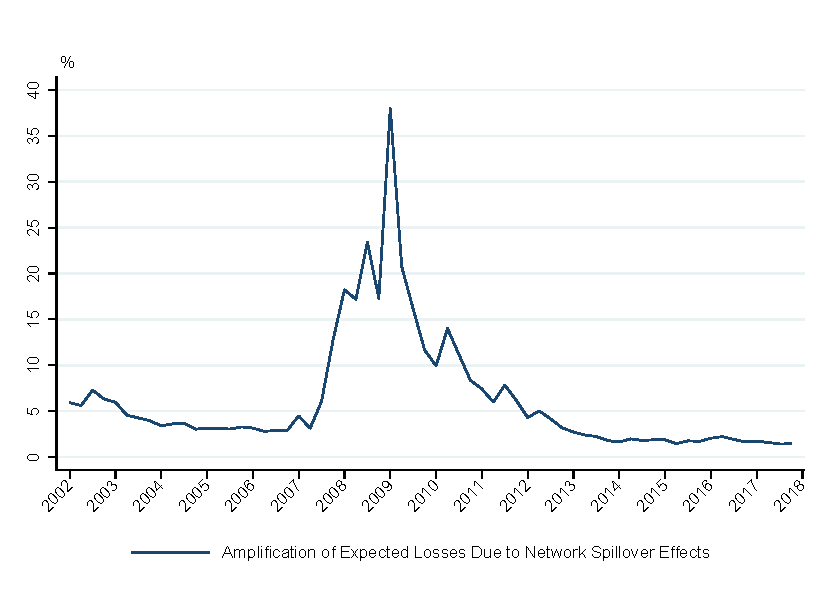
\includegraphics[width=\linewidth, height=0.9\textheight,keepaspectratio]{../output/NVI_benchmark.pdf}
\end{center}

\end{frame}

\begin{frame}

{\Large  Decompositions, robustness}

\end{frame}

\begin{frame}{Both Components are Important} 

\begin{center}
\includegraphics[width=\linewidth, height=0.9\textheight,keepaspectratio]{../output/NVI_components.pdf}
\end{center}

\end{frame}

\begin{frame}{Broker-Dealers Drive Connectivity} 

\begin{center}
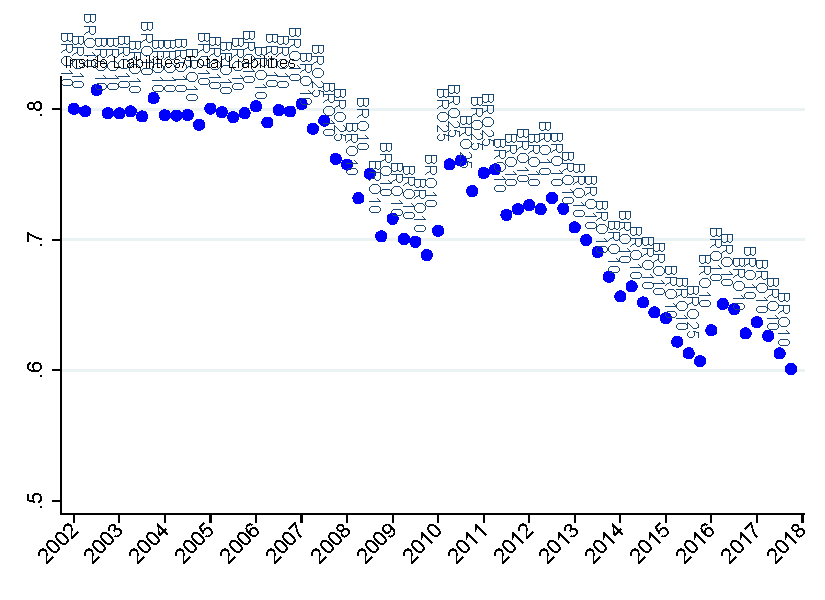
\includegraphics[width=\linewidth, height=0.9\textheight,keepaspectratio]{../output/connectivities_1.pdf}
\end{center}

\end{frame}

\begin{frame}{Ignoring Sectors Underestimates NVI} 
\begin{center}
\includegraphics[width = \textwidth, height=0.9\textheight,keepaspectratio]{../output/delta_externals.pdf} 
\end{center}

\end{frame}

\begin{frame}{`Other' Firm Category, Top Firms by Assets} 
\begin{center}
\begin{table}[htbp] \centering \small
% \def\sym#1{\ifmmode^{#1}\else\(^{#1}\)\fi}F
\input{../output/other}
\end{table}
\end{center}

\end{frame}

\begin{frame}{Individual Node Contagion Index} 
\begin{table}[htbp]\centering \scriptsize
%\def\sym#1{\ifmmode^{#1}\else\(^{#1}\)\fi}
\input{../output/large_instit_breakdowns_clean}
\end{table}

\end{frame}

\begin{frame}{Robustness: Choices for Connectvity} 
\vspace{-0.2in}
\begin{center}
\includegraphics[width = \textwidth, height=\textheight,keepaspectratio]{../output/robustness_beta_selection.pdf} 
\end{center}

\end{frame}

\begin{frame}{Robustness: NVI using Pre- or Post-Crisis EDF}

\begin{center}
\includegraphics[width = \textwidth, height=0.9\textheight,keepaspectratio]{../output/robustness_edf8vs9.pdf} 
\end{center}

\end{frame}


\begin{frame}

{\Large Worst and best networks given empirical data}

\end{frame}

\begin{frame}{Optimizing Network Spillovers}

\begin{figure}
\centering
\begin{minipage}{.5\textwidth}
  \centering
  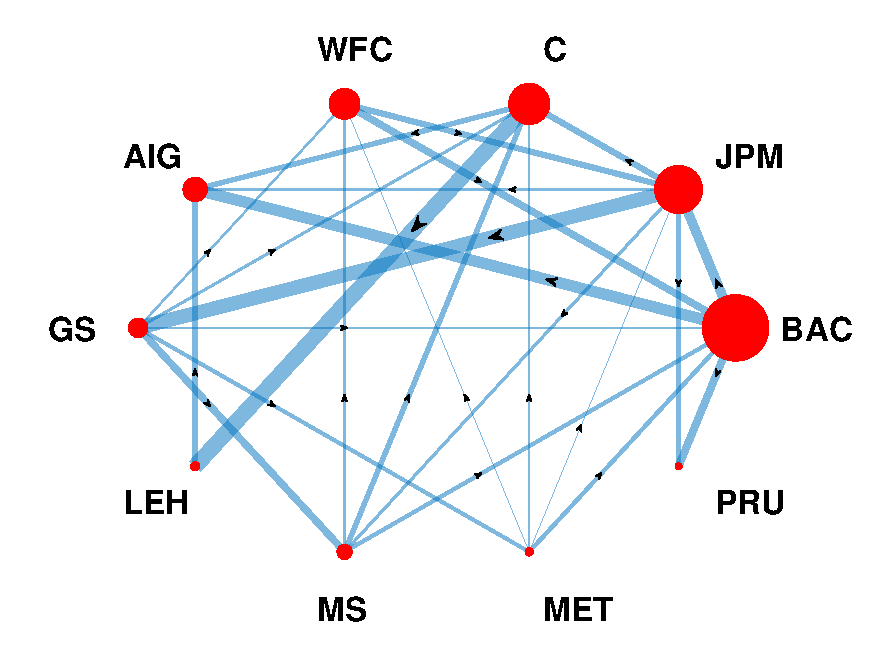
\includegraphics[width=\linewidth]{./worst_10nodes}
  \captionof*{figure}{Maximum Amplification = 2.5\%}
  \label{fig:test1}
\end{minipage}%
\begin{minipage}{.5\textwidth}
  \centering
  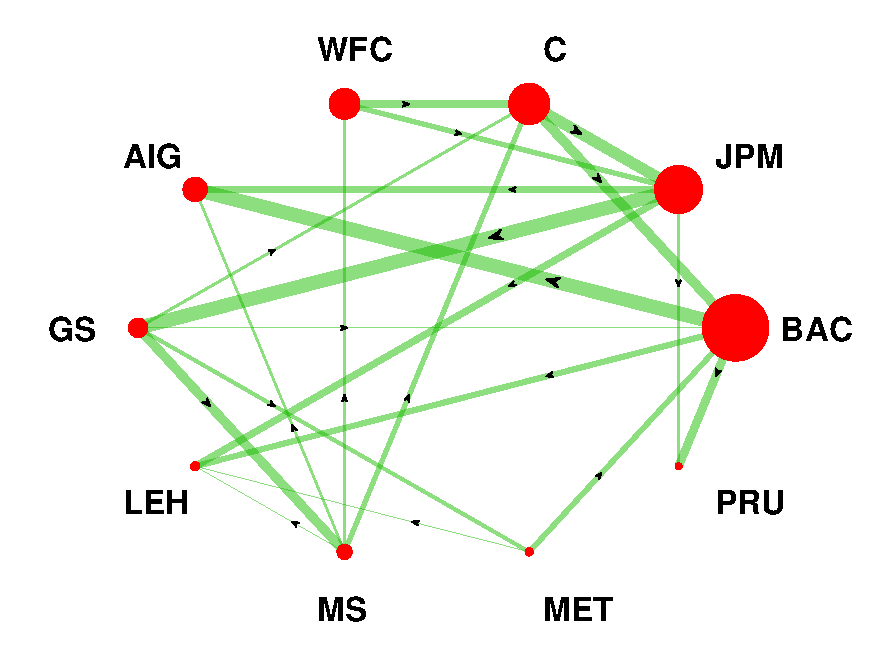
\includegraphics[width=\linewidth]{./best_10nodes}
  \captionof*{figure}{Minimum Amplification = 0.2\%}
  \label{fig:test2}
\end{minipage}
\end{figure}

\end{frame}

\begin{frame}{Conclusion}
\bi
\item First empirical estimate of network default spillovers for entire US financial system
\item Large increase in spillovers during crisis
	\bi
	\item Probabilities of default spiked
	\item Decreasing connectivity mitigated spillovers
	\ei
\item Spillovers outside banks are important
\item Today
	\bi
	\item Vulnerability to spillovers is low
	\item Low probabilities of default
	\item Connectivity of broker-dealers and large BHC low, but increasing in other sub-sectors
	\ei
\ei
\end{frame}

\begin{frame}
 \titlepage

\end{frame}

\begin{frame}

{\Large Appendix: Additional Robustness}

\end{frame}

\begin{frame}{Additional Costs to Bankruptcy, $\gamma$}

\begin{center}
\includegraphics[width = \textwidth, height=0.8\textheight,keepaspectratio]{../output/robustness_gamma.pdf}
\end{center}

\end{frame}

\begin{frame}{Different Classifications of Hard-To-Classify Assets and Liabilities}

\begin{center}
\includegraphics[width = \textwidth, height=0.8\textheight,keepaspectratio]{../output/robustness_perc_unc.pdf}
\end{center}

\end{frame}

\begin{frame}{Using FR-Y15 Data}

\begin{center}
\includegraphics[width = \textwidth, height=0.8\textheight,keepaspectratio]{../output/robustness_nvi_y15.pdf}
\end{center}

\end{frame}
\begin{frame}{Classification of Uninsured Deposits}

\begin{center}
\includegraphics[width = \textwidth, height=0.8\textheight,keepaspectratio]{../output/robustness_y15_depos.pdf}
\end{center}

\end{frame}

\begin{frame}{Extrapolating FR-Y15 Off-Balance Sheet Items}

\begin{center}
\includegraphics[width = \textwidth, height=0.8\textheight,keepaspectratio]{../output/robustness_offbalance.pdf}
\end{center}

\end{frame}

\begin{frame}{Balanced FR-Y9C Panel}

\begin{center}
\includegraphics[width = \textwidth, height=0.8\textheight,keepaspectratio]{../output/robustness_fullsample.pdf} 
\end{center}

\end{frame}

\begin{frame}{Fixed, High Default Probability}

\begin{center}
\includegraphics[width = \textwidth, height=0.8\textheight,keepaspectratio]{../output/nvi_deltafixed.pdf} 
\end{center}

\end{frame}

\end{document}

